\chapter{Diseño para Impresión 3D}

\begin{figure}[H]
	\centering
	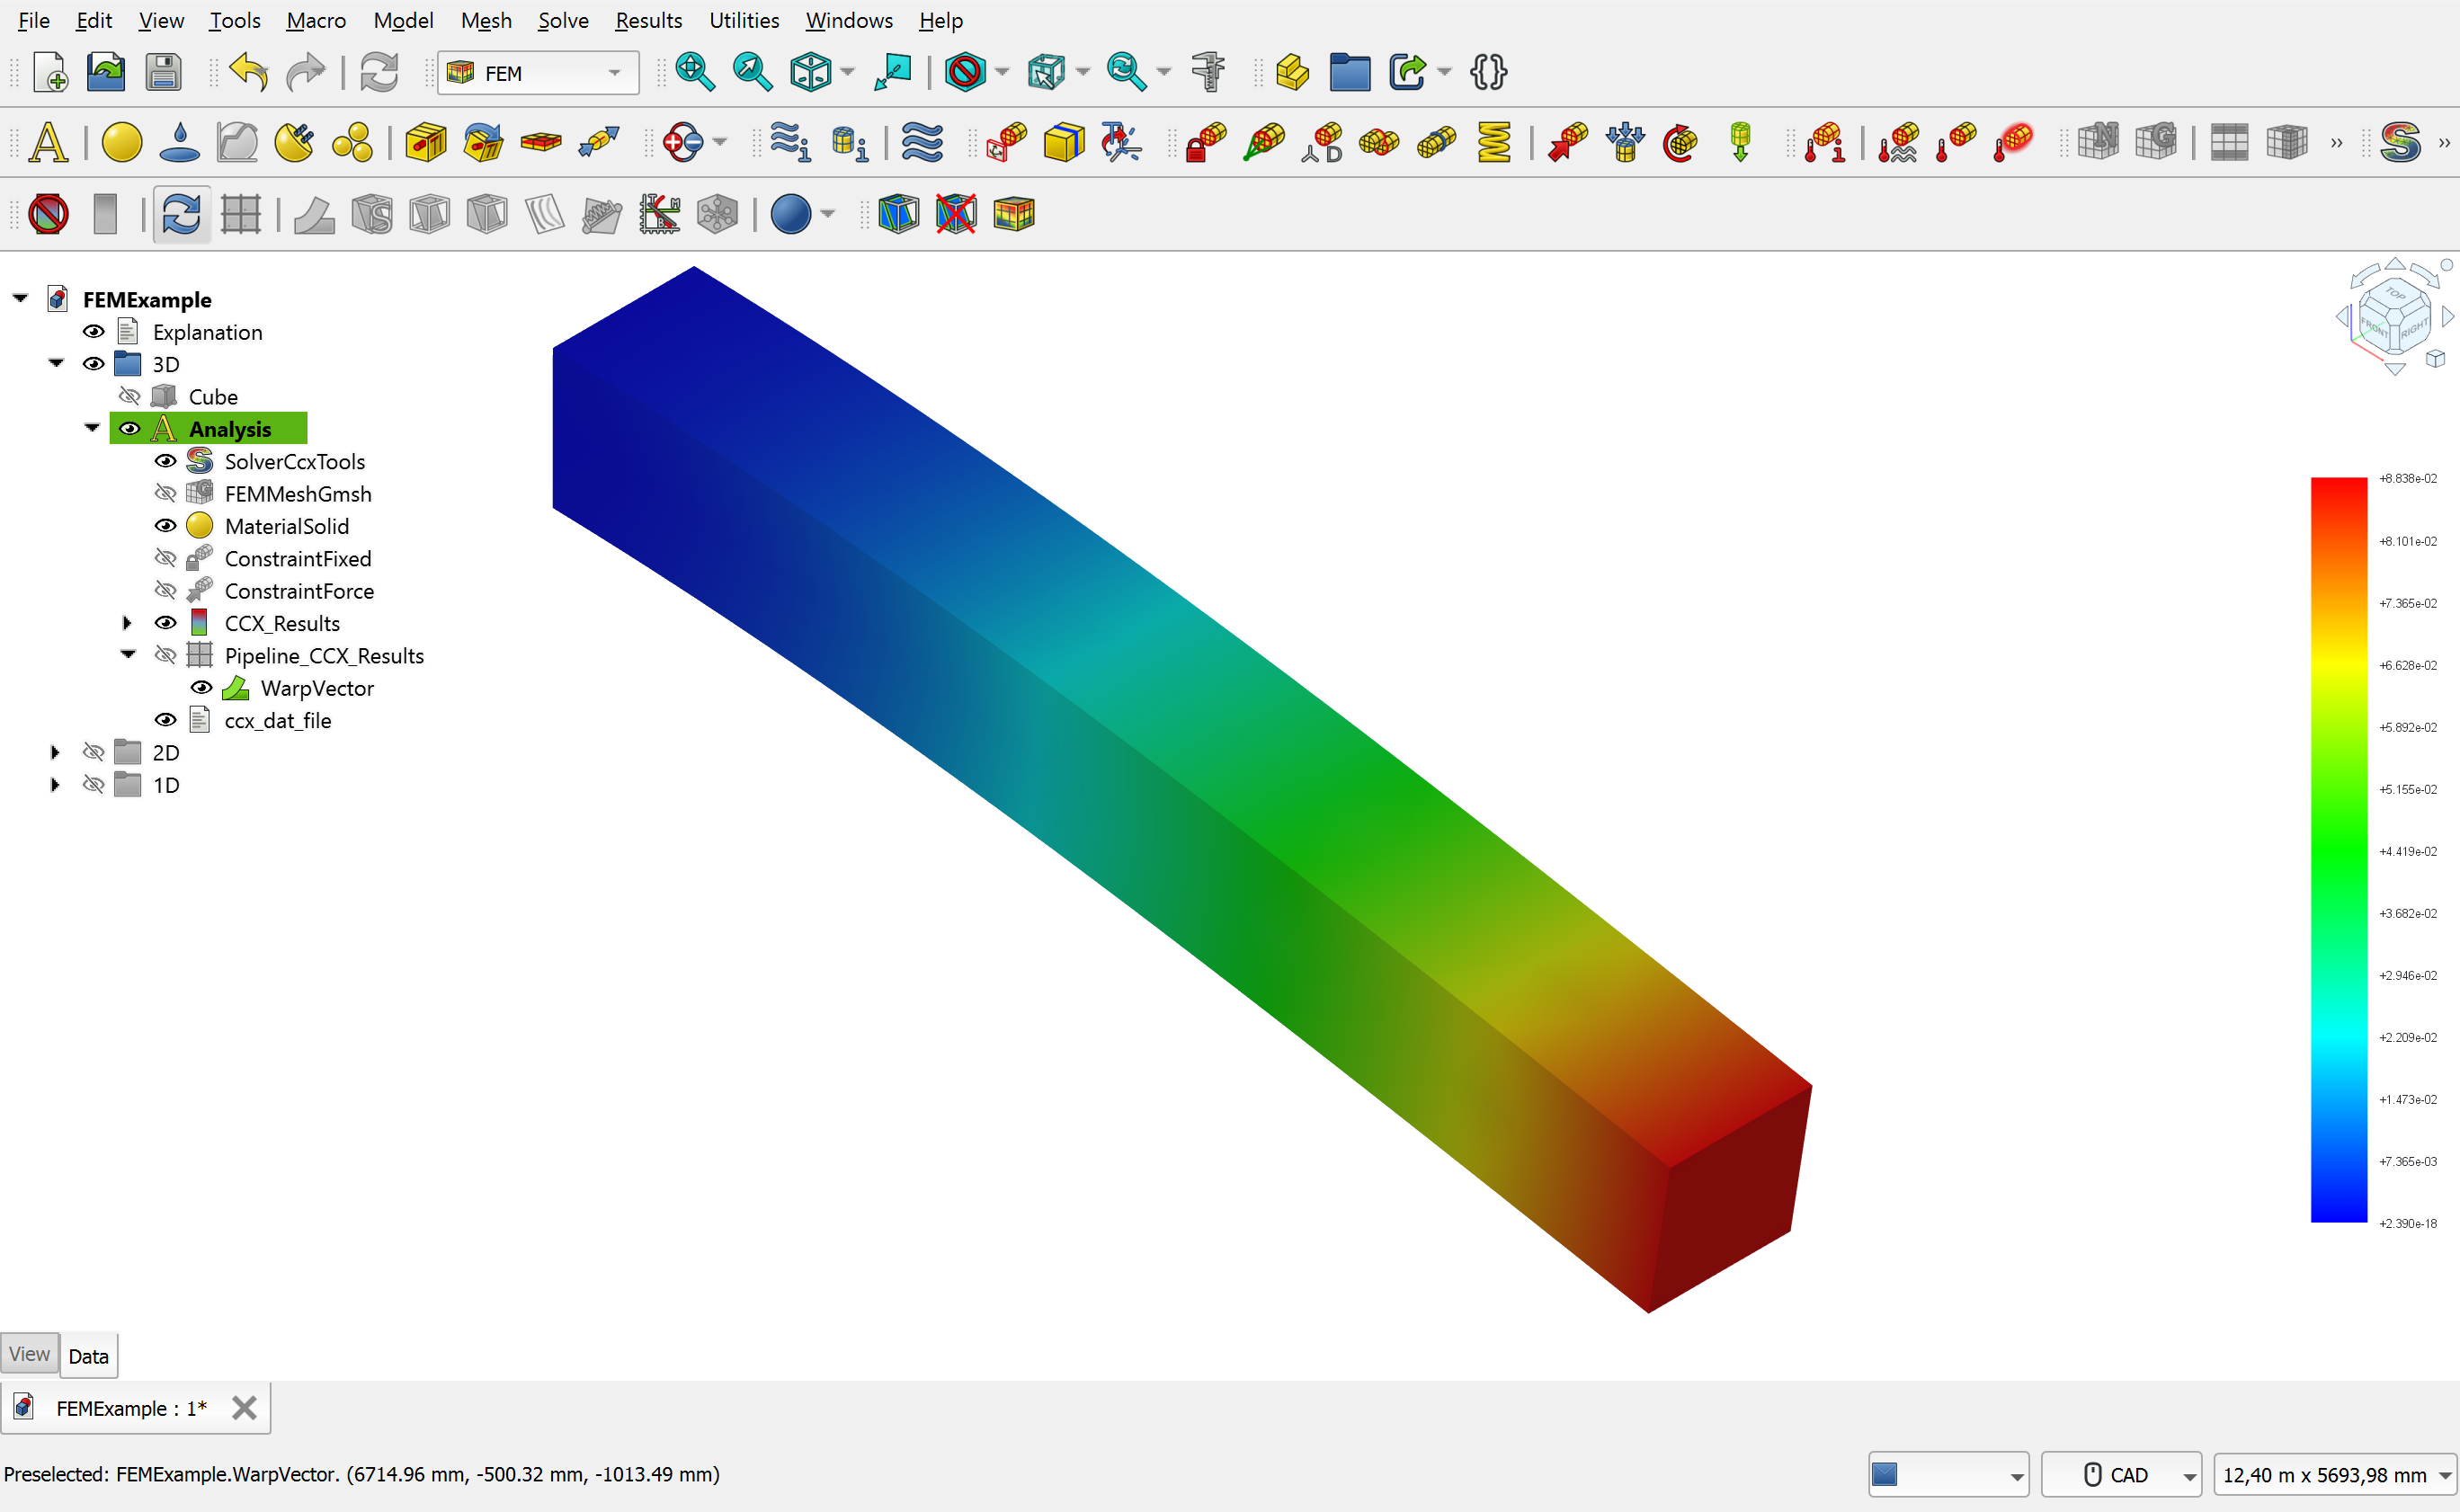
\includegraphics[width=0.8\textwidth]{img/cap10_impresion3d.png}
	\caption{Modelo optimizado para impresión 3D en FreeCAD}
\end{figure}

Aprende a diseñar modelos específicos para impresión 3D.
Optimiza tus diseños para fabricación aditiva y evita
errores comunes de impresión.

%% D. Búsqueda e Inserción de Activos Gráficos
%% Imagen insertada al inicio del capítulo

%% B. Actividades Teóricas
\section{Investigar y responder}
\faPencil

Investiga sobre diseño para impresión 3D y responde:
\begin{enumerate}
	\item ¿Qué es la fabricación aditiva (impresión 3D)?
	\item ¿Qué limitaciones tienen las impresoras 3D?
	\item ¿Cómo se exporta un modelo a formato STL?
	\item ¿Qué es el ``manifold'' y por qué es importante?
	\item ¿Cómo se verifican errores en mallas 3D?
	\item ¿Qué diseños son difíciles de imprimir en 3D?
	\item ¿Cómo se optimizan modelos para reducir tiempo
	      de impresión?
	\item ¿Qué formatos son recomendables para impresión 3D?
\end{enumerate}

%% C. Actividades Prácticas
\section{Resolver los siguientes problemas}
\faWrench

Problemas para aplicar conocimientos:
\begin{enumerate}
	\item Diseña un soporte para teléfono celular optimizado
	      para impresión 3D.
	\item Exporta tu modelo a formato STL y verifica su
	      integridad.
	\item Diseña una pieza con soportes internos para
	      mejorar resistencia.
	\item Crea un modelo con paredes de espesor mínimo
	      recomendado.
	\item Diseña una pieza que evite voladizos pronunciados.
	\item Optimiza un modelo existente reduciendo cantidad
	      de material.
	\item Verifica que tu modelo no tenga huecos internos
	      o errores de malla.
	\item Diseña un encaje tipo ``snap-fit'' para ensamblaje
	      sin pegamento.
	\item Practica el diseño de piezas con texturas o
	      patrones para impresión.
	\item Prepara un modelo para impresión incluyendo
	      orientación y soportes.
\end{enumerate}